
\documentclass[master]{thesis-uestc}

\title{面向长尾分布数据的自监督预训练故障诊断方法研究}{}

\author{王本浩}{Wang Benhao}
\advisor{周雪\chinesespace 教授}{Dr. Xue Zhou}
\school{电子科技大学(深圳)高等研究院}{Shenzhen Institute for Advanced Study}
\major{电子信息}{Electronic and Information Engineering}
\studentnumber{202222280517}

\begin{document}

\makecover

\begin{chineseabstract}
为了适应日益增长的宽带信号和非线性系统的工程应用,用于分析瞬态电磁散射问题的时域积分方程方法研究日趋活跃。本文以时域积分方程时间步进算法及其快速算法为研究课题,重点研究了时间步进算法的数值实现技术、后时稳定性问题以及两层平面波算法加速计算等,主要研究内容分为四部分。

……

\chinesekeyword{时域电磁散射,时域积分方程,时间步进算法,后时不稳定性,时域平面波算法}
\end{chineseabstract}

\begin{englishabstract}
With the widespread engineering applications ranging from broadband signals and non-linear systems, time-domain integral equations (TDIE) methods for analyzing transient electromagnetic scattering problems are becoming widely used nowadays. TDIE-based marching-on-in-time (MOT) scheme and its fast algorithm are researched in this dissertation, including the numerical techniques of MOT scheme, late-time stability of MOT scheme, and two-level PWTD-enhanced MOT scheme. The contents are divided into four parts shown as follows.

\englishkeyword{Time-domain Electromagnetic Scattering, Time-domain Integral Equation, Marching-on In-time (MOT) Scheme, Late-time Instability, Plane Wave Time-domain (PWTD) Algorithm}
\end{englishabstract}

\thesistableofcontents

\chapter{绪\hspace{6pt}论}

\section{研究工作的背景与意义}
旋转机械作为现代工业中的关键机械设备,长期运行在高温、疲劳、重载的复杂环境中。产生的故障可能会造成严重的事故,造成巨大的经济损失和人员伤亡。智能诊断是预测健康管理(PHM)的关键组成部分,PHM是直升机、航空发动机、风力涡轮机、高速列车等各种旋转机械中最重要的系统之一,旨在有效检测故障。传统的智能诊断方法主要包括使用信号处理方法进行特征提取和使用机器学习方法进行故障分类,这些方法已经取得了相当大的进展。然而,面对异构海量数据,由专家设计和选择的特征提取方法和从信号到条件的映射能力在很大程度上取决于先验知识,既费时又需要经验。因此,如何更精确、更有效地进行诊断仍然是一个具有挑战性的问题。

现实生活中的故障检测数据通常服从长尾分布\citing{nanjing2023faultdetection}长尾分布数据是一种偏态分布,即头部类包含了大部分正常数据,相反地,尾部类包含的故障数据量比较少。用长尾数据训练神经网络时,神经网络的性能易被头部类影响而在尾部类上表现较差,对尾部类样本的错分往往会带来更大的损失,对尾部类样本的研究更具有价值意义。因此如何基于长尾分布的故障检测数据训练故障检测模型是一个具有现实意义的难点问题\citing{cumm2023faultdiagnosis}。目前,在视觉识别长尾学习领域有诸多前沿的长尾学习方法,如变分自编码器\citing{kingma2013auto}、生成对抗网络\citing{goodfellow2020generative}、CB(Class-Balanced) Loss\citing{cui2019class}、自监督学习\citing{yang2020rethinking}、MARC决策面调整算法\citing{wang2023margin},而在故障诊断长尾学习领域常见的方案为半监督学习方法\citing{nanjing2023faultdetection}、集成学习\citing{吴亮2023基于多级学习的长尾分布下交通多目标检测}、样本加权\citing{cumm2023faultdiagnosis},少有前者应用前沿的长尾学习方法在故障诊断长尾学习领域。因此,基于前沿的长尾学习方法提出一个适用于故障诊断领域的长尾学习模型是一个具有现实意义的挑战。

目前,大部分神经网络的训练仍然使用的是有监督范式,需要耗费大量的标注数据,标注这些数据是非常耗时费力的。而自监督的提出就是为了打破对人工标注的依赖,即使在没有标注数据的情况下,也可以高效地训练网络。不同于传统的非监督学习,自监督学习通过人工构造输入数据的代理标签,然后依赖于代理标签设计神经网络的监督训练任务。神经网络从而学习到特征表示。文献\cite{zhang2021federated}指出额外的自监督预训练能够使常规的长尾学习算法获得更高的性能,且验证了自监督预训练在CIFAR-LT、ImageNet-LT等视觉识别长尾数据集上的性能提升。目前,在故障诊断长尾学习领域常见的方案为半监督学习方法、集成学习、样本加权,而少有前者应用前沿自监督预训练方法在故障诊断长尾学习领域。因此,基于自监督预训练的长尾数据故障诊断是一个具有现实意义的挑战。

\section{长尾学习方法的国内外研究历史与现状}
\subsection{长尾学习的发展历程和研究现状}
国内外处理长尾问题通常从三个方面入手。一、样本层面,减少样本数量的欠采样如随机欠采样、NearMiss\citing{shen2016near}、ENN\citing{wilson1972asymptotic};增加样本数量的过采样,如随机过采样、SMOTE\citing{chawla2002smote}、变分自编码器\citing{kingma2013auto}、生成对抗网络\citing{goodfellow2020generative}。二、损失函数层面,使用类平衡的损失函数如以数据频率的逆加权\citing{huang2016learning},OHEM(Online Hard Example Mining),Focal Loss\citing{lin2017focal}以及最新的CB(Class-Balanced) Loss\citing{cui2019class}。三、模型层面,如重复组合少数类样本与抽样的同样数量的多数类样本进行集成学习、半监督和自监督学习\citing{yang2020rethinking}、MARC决策面调整算法\citing{wang2023margin}。

目前,基于长尾分布问题,国内外做出了许多研究。例如:Liu J等人\citing{liu2020deep},介绍了一种基于特征云的数据增强手段,从方差较大的数据分布宽广的头部类中学习到类内多样性并转移到尾部类,并应用于人脸识别。Yang Y等人\citing{yang2020rethinking},介绍了不平衡样本的标签在模型训练中的价值,并提出了用半监督的学习方法使用原模型识别无标签的数据,并以获得伪标签的数据扩充原数据集,同时证明了自监督的模型预训练的有效性,且样本维度越高对性能提升越有效。吴磊等人\citing{wu2023personalized}提出了提出一种面向长尾图像的个性化专家识别算法。该算法在残差网络的基础上构建多专家学习网络,并加入个性化学习模块、信息融合模块与个性化信息增强模块,以两阶段的学习方式提升长尾图像整体的识别准确率与中、尾部类别的识别效果。吴亮等人\citing{吴亮2023基于多级学习的长尾分布下交通多目标检测}构建了多级分组分类器,提升尾部类性能的同时,避免头部类性能损失。然后设计了基于多头注意力机制的分组特征重融合模块,为多级分类器输入更精细的特征。最后,基于多级分类器提出了 Logit 联合调整的方法,以缓解组间的不平衡。Wang Y等人\citing{wang2023margin}介绍了一种对长尾视觉识别学习有效的MARC决策面调整算法,对原模型输出的预测分数额外做一次训练——只用三行代码。Cui Y等人\citing{cui2019class},介绍了CB(Class-Balanced)损失函数,在原损失函数上乘以与“独特”样本数量有关的因子从而缓解类别不平衡。CB因子与超参数β有关,平滑了由1到最常见的不平衡因子1∕n。综上,文献\cite{yang2020rethinking}为自监督预训练模型应用在故障诊断长尾学习领域提供了良好的启示,但半监督学习方法在现实的长尾学习模型可能不适用。文献\cite{wu2023personalized,吴亮2023基于多级学习的长尾分布下交通多目标检测}介绍的集成学习方法削弱样本不平衡效应是常规方法,但单个模型在训练时若融合自监督预训练的方法,性能可能会得到提升。文献\cite{wang2023margin}介绍的决策面调整算法对一般的长尾学习模型都适用,但在故障诊断模型上是否可行有待商榷,且该算法对模型性能提升的理论性解释有待完善。文献\cite{cui2019class}介绍的损失函数有着新颖的思路,但超参数β需要人工选择在应用上可能存在难点。以上大部分为学者在视觉长尾学习领域的研究,此类算法在CIFAR-LT、ImageNet-LT等视觉识别数据集取得了较好的效果,而故障诊断长尾学习领域少有前沿的长尾学习算法的应用。因此,前沿的长尾学习算法在故障诊断长尾学习领域的应用具有很高的研究价值。
\subsection{自监督预训练的发展历程和研究现状}
2019 年 MoCo\citing{He_2020_CVPR} 的横空出世,掀起了视觉自监督学习的热潮。后面 SimCLR\cite{chen2020simple}, BYOL\citing{grill2020bootstrap}, SwAV\citing{caron2020unsupervised} 等主流自监督学习算法相继被提出,自监督学习领域呈现出百花齐放,百家争鸣空前繁荣的景象。2021 年末MAE\citing{he2022masked} 更是将自监督学习带到了一个前所未有的新高度。但是繁荣的背后,自监督学习经历了漫长的迭代和发展过程。

目前,对于自监督预训练,国内外做出了许多研究。例如视觉领域:Yang Y等人\citing{yang2020rethinking},介绍了不平衡样本的标签在模型训练中的价值,并提出了用半监督的学习方法使用原模型识别无标签的数据,并以获得伪标签的数据扩充原数据集,同时证明了自监督预训练的有效性,且样本维度越高对性能提升越有效,为自监督预训练在故障诊断长尾学习领域提供了强力的支撑。Doersch C等人\citing{doersch2015unsupervised} 构建了从一张图片中随机抽取两个块,然后让模型来预测一个块相对于另外一个块的位置的自监督预训练任务。Zhang R等人\citing{zhang2016colorful}构建了涂色的自监督预训练任务,将图片转换到 CIE Lab 颜色空间,然后将 L 通道喂入模型,然后让模型去预测 a, b 通道的数值。Gidaris S等人\citing{gidaris2018unsupervised}人为地将图像旋转不同角度,并将旋转角度作为有监督模型训练的代理标签。实验结果表明,该模型可以通过预测旋转角度来学习图像的语义特征,从而为后续任务提供有效的特征表示。无独有偶,近些年在故障诊断领域,自监督预训练的研究也得到了学者们的关注。例如:Zhang T等人\citing{zhang2022prior}建立了以先验知识为代理标签的自监督预训练任务训练卷积自编码器模型,并在小样本学习上得到了应用。Senanayaka等人\citing{senanayaka2020toward}以One-Class SVM输出的标签作为代理标签,使用自监督预训练的卷积神经网络做故障特征提取。W. Zhang等人\citing{zhang2021federated}将时域信号划分为块,通过交换信号块的位置人为制造“伪数据”,自监督预训练的训练目标为区分数据是否为“伪数据”。自监督预训练在视觉学习领域的研究百花齐放,故障诊断领域的研究也蒸蒸日上。综上,文献\cite{doersch2015unsupervised,zhang2016colorful,gidaris2018unsupervised}为视觉领域的自监督预训练方法,应用在故障诊断模型存在困难,但为故障诊断模型的自监督预训练设计提供了思想上的启示。如文献\cite{senanayaka2020toward}的One-Class SVM构造标签在多分类目标上使用聚类算法可能会更有通用性。文献\cite{zhang2021federated}所提的交换信号块的位置预测样本真伪可能与文献\cite{doersch2015unsupervised}的预测图片块的位置可以结合。而文献\cite{zhang2022prior,senanayaka2020toward,zhang2021federated}故障诊断领域的自监督预训练在学习任务上有很大的创新空间,且在长尾学习领域的应用稍有欠缺。因此,故障诊断领域的自监督预训练还处于萌芽阶段,参考视觉领域的前沿自监督学习任务在现有故障诊断领域的自监督预训练方法的基础上提出更具创新性和更高性能的自监督预训练任务是有研究价值和意义的挑战。

\section{本文的主要贡献与创新}
本论文以时域积分方程时间步进算法的数值实现技术、后时稳定性问题以及两层平面波加速算法为重点研究内容,主要创新点与贡献如下:

\section{本论文的结构安排}
本文的章节结构安排如下:

\chapter{长尾学习理论基础与轴承故障数据集}
\section{长尾学习相关理论}
不平衡数据在现实世界中无处不在,大规模数据集通常表现为长尾分布。长尾分布的学习亦是故障诊断领域中常见挑战,例如正常工作状态多,故障工作状态少,或是常见故障状态和罕见故障状态的样本个数差异。现实生活中的故障检测数据通常服从长尾分布,长尾分布数据是一种偏态分布,如图\ref{fig_long_tail}所示,在现实生活中,大规模的训练样本呈现典型的长尾分布,即头部类别的样本个数较多,而尾部类别的样本个数较少,样本个数逐渐降低的分布。用长尾数据训练神经网络时,神经网络的性能易被头部类影响而在尾部类上表现较差,对尾部类样本的错分往往会带来更大的损失,对尾部类样本的研究更具有价值意义。因此如何基于长尾分布的故障检测数据训练故障检测模型是一个具有现实意义的难点问题。
\begin{figure}[h]
    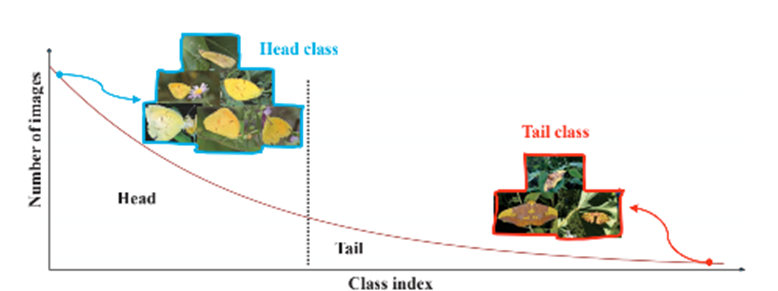
\includegraphics[width=10cm]{long_tail.png}
    \caption{长尾分布示意图}
    \label{fig_long_tail}
\end{figure}

长尾分布的样本具有非常显著的样本不均衡问题,导致训练好的模型易偏向于头部类,从而损害了对尾部类的识别效果。如图\ref{tsne_mean_distribution}所示,样本个数均衡时,各个类别之间具有清晰的区分边界,各类都占据了宽广的特征空间。而当某些类的样本个数减少呈现样本分布失衡的长尾分布时,如图\ref{tsne_lt_distribution}所示,尾部类在特征空间的分布十分狭窄,并依附在头部类附近,从而扭曲了特征空间,损害了类间的多样性和区分性。
这对现代深度学习框架提出了一个重大挑战,即使使用数据重采样方法或类平衡损失等专门技术,在极端类不平衡的情况下,仍然会出现显著的性能下降。因此,为了进一步应对这一挑战,了解类不平衡学习所带来的不同特征至关重要。然而,与平衡数据不同的是,不平衡学习背景下的标签扮演着令人惊讶的有争议的角色,这导致了标签价值的持续困境:一方面,有标签监督的学习算法通常比无监督的学习算法产生更准确的分类器,这表明了标签的积极价值;然而,另一方面,不平衡的标签在学习过程中自然会产生“标签偏差”,其中大多数类别可以显著地驱动决策边界,表明标签的负面影响。因此,不平衡的标签似乎是一把双刃剑。
\begin{figure}[h]
    \subfloat[]{
        \label{tsne_mean_distribution}
        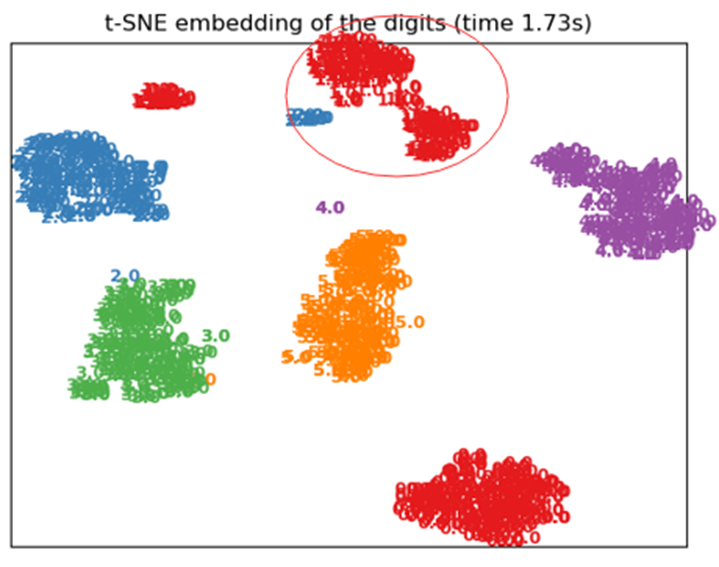
\includegraphics[width=6.77cm]{tsne_mean_distribution.png}
    }
    \subfloat[]{
        \label{tsne_lt_distribution}
        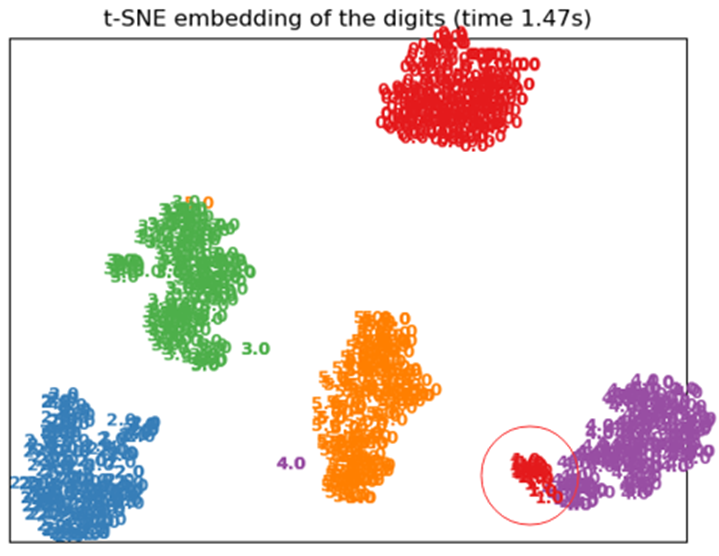
\includegraphics[width=6.77cm]{tsne_lt_distribution.png}
    }
    \caption{均匀/长尾分布数据的tsne图(a)样本均匀分布时的T-SNE分布图;(b)尾部类“1”类样本个为30,头部类样本个数为180个时的T-SNE分布图}
    \label{fig2}
\end{figure}

\section{自监督学习相关理论}
自监督学习是一种范式,利用“代理任务”(pretext)从大规模的无标签数据本身的内在结构挖掘通用的表征信息,通过这种构造的监督信息对网络进行训练,从而可以学习到对下游任务有价值的表征。如图(todo:补充SSL流程框图)所示,自监督学习分为两个阶段:(1)自监督预训练阶段。完全放弃标签信息,专注于数据本身,通过自监督学习进行预训练。从不平衡数据中学习标签不可知的特征表示,减少类别偏差对初始化的影响。(2)微调阶段。使用第一阶段中通过自监督预训练的网络权重作为初始化。在此基础上,可以使用任何标准的不平衡学习技术进行进一步训练,学习最终的分类模型。由于预训练阶段和正常训练阶段是独立的,自监督学习可以与现有的不平衡学习方法无缝结合,增强模型性能,且自监督预训练阶段不依赖标签,使得网络能学习到更通用、更鲁棒的特征表示,从而避免了类别不平衡对特征学习的负面影响。

(todo: 1.补充公式理论Rethinking the Value of Labels for Improving Class-Imbalanced Learning2.补充SSL流程框图)
\section{孪生网络与对比学习相关理论}
\section{相关数据集介绍}

\chapter{基于孪生网络对比学习的自监督预训练方法研究}
\section{引言}
\section{模型整体架构及其模块设计}
\section{实验与分析}
由于时域混合场积分方程是时域电场积分方程与时域磁场积分方程的线性组合,因此时域混合场积分方程时间步进算法的阻抗矩阵特征与时域电场积分方程时间步进算法的阻抗矩阵特征相同。
\section{本章小结}
本章首先研究了时域积分方程时间步进算法的阻抗元素精确计算技术,分别采用DUFFY变换法与卷积积分精度计算法计算时域阻抗元素,通过算例验证了计算方法的高精度。

\chapter{基于K-means聚类的自监督预训练方法研究}
\section{Kmeans介绍}
\section{模型架构}
\section{实验与分析}

\chapter{其他长尾学习方法分析(CB LOSS等)}

\begin{table}[h]
\caption{计算$2m\times 2m$理想导体平板时域感应电流采用的三种存储方式的存储量比较。}
\begin{tabular}{cccc}
\toprule
\multirow{2}{*}{时间步长} & \multicolumn{3}{c}{存储方式} \\
\cmidrule{2-4}
& 非压缩存储方式 & 完全压缩存储方式 & 基权函数压缩存储方式 \\
\midrule
0.4ns & 5.59 MB & 6.78 MB & 6.78 MB\\
0.5ns & 10.17 MB & 5.58 MB & 5.58 MB \\
0.6ns & 8.38MB & 4.98 MB & 4.98 MB \\
\bottomrule
\end{tabular}
\label{tablea}
\end{table}

如图\ref{picd}所示给出了时间步长选取为0.5ns 时采用三种不同存储方式计算的平板中心处$x$方向的感应电流值与IDFT 方法计算结果的比较,……。如图\ref{pice}所示给出了存储方式为基权函数压缩存储方式,时间步长分别取0.4ns、0.5ns、0.6ns时平板中心处$x$方向的感应电流计算结果,从图中可以看出不同时间步长的计算结果基本相同。

\begin{figure}[h]
\subfloat[]{
    \label{picd}
    \includegraphics[width=6.77cm]{picd.pdf}
}
\subfloat[]{
    \label{pice}
    \includegraphics[width=7.04cm]{pice.pdf}
}
\caption{$2m\times 2m$的理想导体平板中心处感应电流$x$分量随时间的变化关系。(a)不同存储方式的计算结果与IDFT方法的结果比较;(b)不同时间步长的计算结果比较比较比较}
\label{fig2}
\end{figure}

由于时域混合场积分方程是时域电场积分方程与时域磁场积分方程的线性组合,因此时域混合场积分方程时间步进算法的阻抗矩阵特征与时域电场积分方程时间步进算法的阻抗矩阵特征相同。

\section{时域积分方程时间步进算法矩阵方程的求解}
\begin{theorem}
如果时域混合场积分方程是时域电场积分方程与时域磁场积分方程的线性组合。
\end{theorem}
\begin{proof}
由于时域混合场积分方程是时域电场积分方程与时域磁场积分方程的线性组合,因此时域混合场积分方程时间步进算法的阻抗矩阵特征与时域电场积分方程时间步进算法的阻抗矩阵特征相同。
\end{proof}
\begin{corollary}
时域积分方程方法的研究近几年发展迅速,在本文研究工作的基础上,仍有以下方向值得进一步研究。
\end{corollary}
\begin{lemma}
因此时域混合场积分方程时间步进算法的阻抗矩阵特征与时域电场积分方程时间步进算法的阻抗矩阵特征相同。
\end{lemma}

\section{本章小结}
本章首先研究了时域积分方程时间步进算法的阻抗元素精确计算技术,分别采用DUFFY 变换法与卷积积分精度计算法计算时域阻抗元素,通过算例验证了计算方法的高精度。

\chapter{全文总结与展望}

\section{全文总结}
本文以时域积分方程方法为研究背景,主要对求解时域积分方程的时间步进算法以及两层平面波快速算法进行了研究。

\section{后续工作展望}
时域积分方程方法的研究近几年发展迅速,在本文研究工作的基础上,仍有以下方向值得进一步研究:

\thesisacknowledgement
在攻读博士学位期间,首先衷心感谢我的导师XXX教授

\thesisappendix

\chapter{中心极限定理的证明}

\section{高斯分布和伯努利实验}


% Uncomment to list all the entries of the database.
% \nocite{*}

\thesisbibliography{reference}

%
% Uncomment following codes to load bibliography database with native
% \bibliography command.
%
% \nocite{*}
% \bibliographystyle{thesis-uestc}
% \bibliography{reference}
%

\thesisaccomplish{publications}

\end{document}
